\part{Topology}
\chapter{$n$-dimensional Euclidean space}
\section{What is $\RR^n$?}
$\RR^n$, as a set, is defined as the set of vertical vectors with n coordinates in the real numbers. Algebraically, $\RR^n$ is a $n$-dimensional vector space over $\RR$; vectors in $\RR^n$ are expressed as vertical vectors:
\[ x=\begin{pmatrix} x_1 \\ x_2 \\ \vdots \\ x_n \end{pmatrix} \]
We usually express the above vector compactly as follows:
\[ x=(x_1,\dots,x_n)^T \]
Since $\RR^n$ is a vector space (over $\RR$), $\RR^n$ has the following extra properties
\begin{itemize}
\item For any two vectors $x,y$ we may perform addition
\[ x+y=(x_1+y_1,\dots,x_n+y_n)^T \]
Properties of addition:
\begin{enumerate}
\item $x+y=y+x$
\item $(x+y)+z=x+(y+z)$
\item Zero vector $0=(0,\dots,0)$ satisfies $x+0=0+x=x$
\item For any vector $x$, its negative $-x$ satisfies $x+(-x)=(-x)+x=0$
\end{enumerate}
\item For any vector $x$ and real number (scalar) $k$ we may perform scalar multiplication
\[ kx=(kx_1,\dots,kx_n)^T \]
Properties of scalar multiplication:
\begin{enumerate}
\item $0\cdot x=0,1\cdot x=x$
\item $(kl)x=k(lx)=l(kx)$
\item $k(x+y)=kx+ky$
\item $(k+l)x=kx+lx$
\end{enumerate}
\end{itemize}

These properties make up the algebraic structure of $\RR^n$, which may then be further expanded in linear algebra. However, in this section we shall focus on the analytical/topological aspects of Euclidean space.

So what's the difference? The Euclidean space is something that builds upon the vector space $\RR^n$. Specifically speaking, it is $\RR^n$ endowed with two extra notions:
\begin{itemize}
\item The \textbf{norm} of the Euclidean space $\norm{\cdot}$ is a real-valued function $\norm{\cdot}:\RR^n\to\RR$. Given a vector $x=(x_1,\dots,x_n)^T$ in $\RR^n$, the norm of $x$ is defined as
\[ \norm{x}\coloneqq\sqrt{\sum_{i=1}^nx_i^2}=\sqrt{x_1^2+\cdots+x_n^2}. \]
\item The \textbf{metric} $d$ of the Euclidean space is a real-valued function $d:\RR^n\times\RR^n\to\RR$. Given two vectors $x=(x_1,\dots,x_n)^T$ and $y=(y_1,\dots,y_n)^T$, the distance between $x$ and $y$ is defined as
\[ d(x,y)\coloneqq\norm{x-y}=\sqrt{\sum_{i=1}^n(x_i-y_i)^2}=\sqrt{(x_1-y_1)^2+\cdots+(x_n-y_n)^2}. \]
\end{itemize}

As you can see here, the norm is something like the length of the vector itself (distant to the origin; absolute value in the case of $\RR^1$). The \textbf{metric} on the other hand refers to the distance function which measures the length between two points in $\RR^n$ (determined by their positional vectors $x$ and $y$). Now these two notions may seem similar to each other, but in fact they are pretty asymmetrical. Essentially, the metric is a much more general notion than the norm: the norm can only be defined on vector spaces; the metric can literally be defined on any set.

Before explaining this, we will look at the fundamental properties of the norm and the metric. In fact, these properties are precisely the definition of a norm over some random vector space, and of a metric over some random set.
\begin{remark}
Note that the definitions for norm and metric depends on the space; in the above definitions the algebraic expression defining these two are only applicable to Euclidean spaces, and in fact they define what an Euclidean space should be, lengths intuitive to our common perception.
\end{remark}

Norms are required to satisfy the following:
\begin{enumerate}
\item \textbf{Positive Definiteness}: For any vector $x$, $\norm{x}\ge0$, and $\norm{x}=0$ if and only if $x=0$.
\item \textbf{Absolute Homogeneity}: For any vector $x$ and scalar $a$, $\norm{ax}=|a|\cdot\norm{x}$.
\item \textbf{Subadditivity (Triangle Inequality)}: For any two vectors $x$ and $y$, $\norm{x+y}\le\norm{x}+\norm{y}$.
\end{enumerate}

Metrics are required to satisfy the following:
\begin{enumerate}
\item \textbf{Positive Definiteness}: For any two elements $x$ and $y$, $d(x,y)\ge0$, and $d(x,y)=0$ if and only if $x=y$.
\item \textbf{Symmetry}: For any two elements $x$ and $y$, $d(x,y)=d(y,x)$.
\item \textbf{Triangle Inequality}: For any three elements $x$,$y$ and $z$, $d(x,z) \le d(x,y)+d(y,z)$.
\end{enumerate}

Generally, if there is a norm $\norm{\cdot}$ on some random vector space, then this norm naturally determines a metric $d(x,y)=\norm{x-y}$, which is precisely the case for Euclidean spaces.

\section{Concepts in Euclidean Space}
\subsection{Bounded Sets}
\begin{defn}{Bounded set}{}
A set $E$ in $\RR^n$ is called a \vocab{bounded set} if there exists $M>0$ such that $\norm{x}\le M$ for all $x$ in $E$.
\end{defn}

\begin{exmp}{}{}
Given $E$ and $F$ in $\RR^n$ and real number $k$, define
\[ kE=\{kx \mid x\in E\} \]
\[ E+F=\{x+y \mid x\in E,y\in F\} \]
\begin{enumerate}[label=(\alph*)]
\item Show that if $E$ is bounded, then $kE$ is bounded;
\item Show that if $E$ and $F$ are bounded, then $E+F$ is bounded.
\end{enumerate}
\end{exmp}

\subsection{Diameter}
\begin{defn}{Diameter}{}
Given a set $E\subset\RR^n$, the \vocab{diameter} of $E$ is defined as
\[ \diam E=\sup_{x,y\in E}d(x,y). \]
\end{defn}

\begin{exmp}{}{}
Find the diameter of the open unit ball in $\RR^n$ given by
\[ B=\{x\in\RR^n \mid \norm{x}<1\}. \]
\end{exmp}
\begin{solution}
First note that
\[ d(x,y)=\norm{x-y}\le\norm{x}+\norm{-y}=\norm{x}+\norm{y}<1+1=2. \]
On the other hand, for any $\epsilon>0$, we pick
\[ x=\brac{1-\frac{\epsilon}{4},0,\dots,0}, \quad y=\brac{-\brac{1-\frac{\epsilon}{4}},0,\dots,0}. \]
Then $d(x,y)=2-\dfrac{\epsilon}{2}>2-\epsilon$.

Therefore $\diam B = 2$.
\end{solution}

\begin{exmp}{}{}
Given a set $E$ in $\RR^n$, show that $E$ is bounded iff $\diam E<+\infty$.
\end{exmp}
\begin{proof}
\textbf{Forward direction:}

If $E$ is bounded, then there exists $M>0$ such that $\norm{x}\le M$ for all $x \in E$.

Thus for any $x,y \in E$,
\[ d(x,y)=\norm{x-y}\le\norm{x}+\norm{y}\le2M. \]
Thus $\diam E = \sup d(x,y) \le 2M<+\infty$.

\textbf{Backward direction:}

Suppose that $\diam E=r$. Pick a random point $x \in E$, suppose that $\norm{x}=R$.

Then for any other $y \in E$,
\[ \norm{y}=\norm{x+(y-x)}\le\norm{x}+\norm{y-x}\le R+r. \]
Thus, by picking $M=R+r$, we obtain $\norm{y}\le M$ for all $y \in E$, and we are done.

\begin{remark}
Basically you use $x$ to confine $E$ within a ball, which is then confined within an even bigger ball centered at the origin.
\end{remark}
\end{proof}

\subsection{Distance Between Sets}
\begin{defn}{Distance between sets}{}
Given two sets $E,F\subset\RR^n$, the \vocab{distance between sets} $E$ and $F$ is defined as
\[ d(E,F)=\inf_{x\in E,y\in F}\norm{x-y}. \]
\end{defn}

Obviously $d(E,F)>0$ implies that $E$ and $F$ are disjoint, but $E$ and $F$ may still be disjoint even if $d(E,F)=0$. For example, the closed intervals $E=(-1,0)$ and $F=(0,1)$.

\begin{exmp}{}{}
Suppose that $E$ and $F$ are sets in $\RR^n$ where $E$ and $F$ is finite. Prove that $E$ and $F$ are disjoint iff $d(E,F)>0$.
\end{exmp}

\section{Topology in Euclidean Space}
Before we move on, we need to talk about how we think about topology. The concept first begins with an attempt to say that two points are close to one another. Of course, we did define the metric earlier, But as it turns out, this particular notion can be made extremely abstract. Specifically speaking, we could theoretically define closeness simply with set theory.

\begin{defn}{Neighbourhood basis}{}
Given a set $X$, we define a family of subsets in $X$, denoted by $\mathcal{B}$, to describe points close to each other; points that belong to the same set $U$ in $\mathcal{B}$ are considered to be close to each other w.r.t. $U$.
\end{defn}

\begin{defn}{Neighbourhood}{}
Given a point $x \in X$, we use the term neighbourhood to describe a particular construction for $x$; $N$ is said to be a neighbourhood of $x$, if there exists $U$ in $\mathcal{B}$ containing $x$ such that $U$ is a subset of $N$.
\end{defn}

\begin{defn}{Neighbourhood system}{}
Given a point $x \in X$, the neighbourhood system of $x$, denoted by $\mathcal{N}(x)$, is the set of all neighbourhoods of $x$.
\[ N\in\mathcal{N}(x) \iff \exists U\in\mathcal{B} \suchthat x\in U\subset N \]
\end{defn}

There are still some problems regarding the above definitions.
\begin{itemize}
\item If $M$ and $N$ are neighbourhoods of $x$, is $M\cap N$ a neighbourhood of $x$?

Supposedly the answer should be yes, because $M$ and $N$ should contain all the points that are close to $x$.

\item If $y$ is close to $x$ w.r.t. $N$, then supposedly the points in $N$ should contain points close to $Y$ as well.

There are some of the more basic requirements, such as $x$ must have a way to define closeness so there must be a neighbourhood containing $x$ (even if it's just one set $\{x\}$, which sort of implies that every other element is far away from $x$).
\end{itemize}

People realised that the above requirements can be formalised simply with the neighbourhood systems themselves 

These are the axioms for the neighbourhood systems:
\begin{enumerate}
\item $\mathcal{N}(x)$ is nonempty, and for all $U\in\mathcal{N}(x)$, $x\in U$.
\item If $U,V\in\mathcal{N}(x)$, then there exists $W\in\mathcal{N}(x)$ such that $W$ is a subset of $U\cap V$.
\item If $U\in\mathcal{N}(x)$ and $y\in U$, then there exists $V\in\mathcal{N}(y)$ such that $V$ is a subset of $U$.
\end{enumerate}

As for the Euclidean plane, we have a natural way of defining the neighbourhood systems. First we pick the neighbourhood basis to be
\[ \mathcal{B} = \{B(x,\epsilon) \mid x\in\RR^n,\epsilon>0\} \]
Then we say that $N$ is a neighbourhood of $x$ if there exists $\epsilon>0$ such that $B(x,\epsilon)$ is in $N$.

$B(x,\epsilon)$ represents the points close to $x$, whereas a neighbourhood $N$ of $x$ should contain all the points close to $x$, at least from the perspective of $B(x,\epsilon)$.

Once we have neighbourhood systems, we can then define the two most important kinds of sets in topology, open and closed sets.

(In topology, we actually define open and closed sets with axioms first and then define neighbourhoods from there, but this definition is very opaque and will only be revised in the far future.)

\begin{itemize}
\item Basic constructions

A \textbf{ball} in $\RR^n$ is determined by its center $x\in\RR^n$ and its radius $r>0$, denoted by $B(x,r)$.

A \textbf{punctured ball} in $\RR^n$ is a ball excluding its center, denoted by $B_0(x,r)$.

\item Neighbourhood, interior and open sets

A set $A\subset\RR^n$ containing $x$ is called a \textbf{neighbourhood} of $x$ if $B(x,\epsilon)\subset A$ for some $\epsilon>0$.

An element $x\in A$ is called an \textbf{interior point} if $A$ is a neighbourhood of $x$.

The \textbf{interior} of a set $A$, denoted by $A^\circ$, is the set of all interior points in $A$.

A set $A\subset\RR^n$ is called an \textbf{open set} if $A^\circ=A$, i.e. all points in $A$ are interior points.

\item Limit points, closure and closed sets

An element $x\in A$ is called a limit point of $A$ if $B_0(x,\epsilon)\cap A\neq\emptyset$ for all $\epsilon>0$.

The induced set of a set, denoted by $A^\prime$, is the set of all limit points of $A$.

The closure of a set $A$, denoted by $\bar{A}$, is the union set $A\cup A^\prime$.

A set $A\subset RR^n$ is called a closed set if $\bar{A}=A$, i.e. all limit points of $A$ are contained in $A$

\item Further topological constructions of points

An element $x\in A$ is called an isolated point of $A$ if it is not a limit point of $A$.

The boundary of a set $A$, denoted by $\partial A$, is the set difference $\bar{A}\setminus A^\circ$.

An element $x\in\RR^n$ is called a boundary point of $A$ if it is in $\partial A$.

An element $x\in\RR^n$ is called an exterior point of $A$ if it is an interior point of $A^c$.

\item Further topological constructions of sets

A set $A\subset\RR^n$ is compact if it is a bounded closed set.

A subset $B\subset A$ is called a dense subset of $A$ if $\bar{B}=A$.

A set $A\subset\RR^n$ is nowhere dense its closure has no interior, i.e. $(\bar{A})^\circ=\emptyset$.
\end{itemize}

In general topology, these are the axioms used to define open and closed sets. At the moment we only consider them to be certain properties regarding open and closed sets in $\RR^n$.
\begin{enumerate}[label=\textbf{P\arabic*}]
\item $A$ is open if and only if $A^c$ is closed.

\begin{proof}
\textbf{Forward direction}:
Let $A$ be open, we consider the punctured balls of $x \notin A$ (if $x \notin A$, we consider the punctured balls centered at $x$).

Our goal is to show that $B_0(x,r)$ always intersects with $A^c$

So suppose otherwise that $B_0(x,\epsilon)$ is a subset of A for some $\epsilon>0$

Ah no sorry, we consider x not in $A^c$

The thing is we want to show that $A^c$ is closed, i.e. all limit points of $A^c$ are in $A^c$

So suppose otherwise that $x$ is a limit point of $A^c$ that is not in $A^c$

$x$ is a limit point of $A^c$, hence for all $\epsilon>0$, $B_0(x,\epsilon)$ always intersects with $A^c$

This is equivalent to saying that $B_0(x,\epsilon)$ is never a subset of $(A^c)^c=A$

However, $x$ is not in $x \notin A^c$, so $x \in A$.

But if A is open, then there exists $\epsilon>0$ such that $B(x,\epsilon)$ is a subset of $A$, a contradiction

\textbf{Backward direction}: Let $A^c$ be closed. Suppose otherwise that $A$ is not open, i.e. there is a point $x\in A$ such that $B(x,\epsilon)$ is never a subset of $A$; that is to say, $B(x,\epsilon)$ always intersects with $A^c$

Since $x \in A$, then $B(x,\epsilon) \cap A^c = B_0(x,\epsilon) \cap A^c$

But this means that $B_0(x,\epsilon) \cap A^c$ is never empty, hence $x$ is a limit point of $A^c$.

However, $x \in A$, contradictory to $A^c$ being closed and thus should contain all of its limit points
\end{proof}

\item An arbitrary union of open sets is open; a finite intersection of open sets is open.

\begin{proof}
Let $A$ be an arbitrary union of open sets $\{U_i\}_{i \in I}$.

Then for any $x \in A$, suppose that $x \in U_i$, then since $U_i$ is open we can pick $B(x,\epsilon)$ subset of $U_i$ subset of $A$

On the other hand, let $U$ and $V$ be open sets and let $x \in U \cap V$. 
Since $U$ and $V$ are open, we can pick $\epsilon_1$ and $\epsilon_2$ such that $B(x,\epsilon_1)$ is in $U$ whereas $B(x,\epsilon_2)$ is in $V$. 
Then we simply pick $\epsilon=\min\{\epsilon_1,\epsilon_2\}$ so that $B(x,\epsilon)$ is in $U \cap V$.
\end{proof}

\item An arbitrary intersection of closed sets is closed; a finite union of closed sets is closed.

\begin{proof}
This follows from de Morgan's Law on P1 and P2.
\end{proof}
\end{enumerate}

\begin{prbm}\label{sizes}
Compare the sizes of the following pairs of sets, i.e. determine if they are equal, or if one set may be a subset of the other.
\begin{enumerate}
\item $(A\cup B)^\circ$, $A^\circ\cup B^\circ$
\item $(A\cap B)^\circ$, $A^\circ\cap B^\circ$
\item \label{size} $\overline{A\cup B}$, $\bar{A}\cup\bar{B}$
\item $\overline{A\cap B}$, $\bar{A}\cap\bar{B}$
\end{enumerate}
\end{prbm}

\begin{proof} \
\begin{enumerate}
\item $(A\cup B)^\circ$ may be bigger

In $\RR$ we consider the intervals $A=(-1,0]$ and $B=[0,1)$, then
\[ A^\circ\cup B^\circ=(-1,0)\cup(0,1), \quad (A\cup B)^\circ=(-1,1) \]

For $x \in A^\circ \cup B^\circ$, we have either $x \in A^\circ$ or $x \in B^\circ$, so there is some ball centered at $x$ that is contained in either $A$ or $B$ and thus must be contained in $A\cup B$ as well.

\item Equal

If $x \in (A\cap B)^\circ$, then there exists a ball $U$ centered at $x$ such that $U$ is in both $A$ and $B$, so $x$ is in both $A^\circ$ and $B^\circ$.

On the other hand, $A^\circ\cap B^\circ$ is a subset of $A\cap B$; taking the interior of both sides, then since the intersection between two open sets is open we find that $A^\circ\cap B^\circ$ is a subset of $(A\cap B)^\circ$.

\item Equal

\item $\bar{A}\cap\bar{B}$ may be bigger
\end{enumerate}
\end{proof}

\begin{prbm}
Prove that the set of exterior points, $(A^c)^\circ$ is the same as $(\bar{A})^c$.
\end{prbm}

\begin{proof}
\begin{align*}
x \in (A^c)^\circ 
&\iff \exists \epsilon>0 \text{ such that } B(x,\epsilon) \subset A^c \\
&\iff B(x,\epsilon) \cap A = \emptyset \\
&\iff x \notin A \text{ and } B_0(x,\epsilon) \cap A=\emptyset \\
&\iff x \notin A \cup A^\prime = \bar A \\
&\iff x \in (\bar A^c)
\end{align*}
\end{proof}

\begin{prbm}
Regarding alternative descriptions:
\begin{enumerate}
\item $A$ is a neighbourhood of x if and only if there exists an open set U such that x is in U, U is subset of A (trivial except you'll actually need to prove that balls are open sets).
\item If $x$ is a limit point of $A$, then in fact for any $\epsilon>0$, $B(x,\epsilon)$ contains infinitely many elements of $A$ (you don't need to mention the punctured ball here because of obvious reasons; converse is trivial but a good and intuitive description).
\item $x$ is a boundary point of $A$ if and only if for all $\epsilon>0$, $B(x,\epsilon)$ intersects with both $A$ and $A^c$.
\end{enumerate}
\end{prbm}

\begin{proof} \
\begin{enumerate}
\item We show that $B(x,\epsilon)$ is open:

$\forall y \in B(x,\epsilon)$, 
\[ |y-x|<\epsilon \]

$\forall z \in B(y,\epsilon-|y-x|)$, 
\[ |z-x|\le|z-y|+|y-x|<\epsilon-|y-x|+|y-x|=\epsilon \]

$\therefore\:B(y,\epsilon-|y-x|) \subset B(x,\epsilon)$

\item We construct a sequence $\{x_n\}$ recursively as follows:
\begin{itemize}
\item Pick $x_1 \in B_0(x,\epsilon) \cap A$
\item Pick $x_{n+1} \in B_0(x,|x_n-x|) \cap A$
\end{itemize}
It is easy to see that the balls above are getting smaller so all $x_n$ are both mutually distinct and all contained in $B(x,\epsilon)$.

\item $x$ is a boundary point if and only if $x \in \bar{A} \setminus A^\circ$

\textbf{Forward direction}: 

We consider two cases
\begin{itemize}
\item $x \in A$, then all $B(x,\epsilon)$ intersects with $A$ at $x$, but since x is not in $A^\circ$ they must always intersect with $A^c$ as well.
\item $x \notin A$, then all $B(x,\epsilon)$ intersect with $A^c$ at $x$, but since $x \in \bar{A}$, $x$ is a limit point of $A$ and thus $B(x,\epsilon)$ always intersects with $A$.
\end{itemize}

\textbf{Backward direction}:

We consider two cases
\begin{itemize}
\item $x \in A$, then since $B(x,\epsilon)$ always intersects with $A^c$, $x$ cannot be in $A^\circ$.
\item $x \notin A$, then since $B(x,\epsilon)$ always intersects with $A$, $x$ must be in $\bar{A}$.
\end{itemize}

In fact we can describe the closure without referring to punctured balls and induced sets:
$x \in \bar{A}$ if and only if $B(x,\epsilon)$ always intersects with $A$

Also as a side note, $A\circ\cup \partial A\cup (A^c)\circ=\RR^n$
\end{enumerate}
\end{proof}

\begin{prbm}
Regarding closures (The following properties are relatively nontrivial compared to its 'open-set' counterparts):
\begin{enumerate}[label=(\alph*)]
\item $A^\prime$ is closed.
\item $\bar{A}$ is closed, i.e. bar(barA)=barA
\end{enumerate}
\end{prbm}

\begin{proof} \
\begin{enumerate}[label=(\alph*)]
\item In order to show that $A^\prime$ is closed, we need to show that if $x$ is a limit point of $A^\prime$, then $x\in A^\prime$, i.e. $x$ is a limit point of $A$.

So we need to show that limit points of $A^\prime$ are always limit points of $A$: 
Let $x$ be a limit point of $A^\prime$, then for all $\epsilon>0$, $B_0(x,\epsilon/2)$ intersects with $A^\prime$ and we may pick $y \in B_0(x,\epsilon/2)\cap A^\prime$

Now here's the tricky part
Since $y \in A^\prime$, y is a limit point of $A$, hence $B_0(y,|y-x|)$ intersects with $A$ and thus we may pick $z \in B_0(y,|y-x|)\cap A$.

We show that $z \in B_0(x,\epsilon)$:
\[ |z-x|\le|z-y|+|y-x|<2|y-x|<\epsilon, \]
hence $z \in B(x,\epsilon)$.
\[ |z-y|<|x-y|, \]
hence $z \neq x$

$\therefore\:z \in B_0(x,\epsilon)$

\item As for (b), it is just (a) and \cref{sizes} \cref{size}.
\end{enumerate}
\end{proof}

For homework, you'll work out some properties regarding dense sets

1. $A$ is a dense set in $X$ if and only if $A$ intersects with all open sets in $X$.
2. If $A$ is dense in $X$ and $B$ is dense in $A$, then $B$ is dense in $X$
3. If $A$ and $B$ are dense in $X$ where $A$ is open, then $A\cap B$ is dense in $X$

\section{Important Theorems}
\begin{thrm}{Cantor's Intersection Theorem}{}
Given a decreasing sequence of compact sets $A_1\supset A_2 \supset \cdots$, there exists a point $x\in\RR^n$ such that $x$ belongs to all $A_i$. In other words, $\bigcap_{i=1}^\infty A_i\neq\emptyset$. Moreover, if for all $i\in\NN$ we have $\diam A_{i+1}\le c\cdot\diam A_k$ for some constant $c<1$, then such a point must be unique, i.e. $\bigcap_{i=1}^\infty A_k=\{x\}$ for some $x\in\RR^n$.
\end{thrm}

\begin{thrm}{Heine--Borel Theorem}{}
A set $A\subset\RR^n$ is compact if and only if every open covering has a finite subcover, i.e. for any family of open sets $\mathscr{U}=\{U_i\}_{i\in I}$ satisfying $A\subset\bigcup_{i\in I}U_i$, there exists $\{U_1,\dots,U_n\}\subset\mathscr{U}$ such that $A\subset\bigcup_{i=1}^n U_i$.
\end{thrm}

\begin{thrm}{Bolzano--Weierstrass Theorem}{}
Infinite bounded sets in $\RR^n$ must contain limit points.
\end{thrm}

We will follow a very specific sequence of steps to prove these three theorems:
\begin{enumerate}[label=(\alph*)]
\item Cantor Intersection for $n=1$
\item Bolzano--Weierstrass for $n=1$
\item Bolzano--Weierstrass for general $n$
\item Cantor Intersection for general $n$
\item Heine--Borel for general $n$
\end{enumerate}

\begin{proof} \
\begin{enumerate}[label=(\alph*)]
\item Suppose that there is a decreasing sequence of compact sets $A_1, A_2, \dots$ in the real numbers

Since $A_k$ are bounded, we may let $a_k=\inf A_k$
Also since $A_k$ are closed, $a_k \in A_k$

Note that since $A_k$ is a decreasing sequence of sets we have $a_1\le a_2\le\dots$

Also, whenever we have $n>k$, we have $a_n \in A_n$, but $A_n \subset A_k$ and thus $a_n \in A_k$.

Let $b_1=\sup A_1$, then $a_k \in A_1$ and thus $a_k\le b_1$ for all $k$.

This tells us that the sequence $\{a_k\}$ is bounded above, and thus we may let $a=\sup a_k$.

Our goal is to show that the number $a$ appears in all $A_k$, thus showing that the entire intersection $\bigcap A_k$ contains $a$ and thus must be non-empty.

Now we split this in two cases, which asks whether a is simply made from isolated points, or if it is actually some nontrivial point obtained from the boundaries of $A_k$

\textbf{Case 1:} $a_k=a$ for some $k$
In this case we see that $a_k\le a_n\le a$ for all $n>k$ and thus $a_n=a$ in this case, therefore a is an element in $A_n$ for all $n$

In this case you can imagine that there is a possibility where a is an isolated minimum point of $A_n$ which stays there forever in the decreasing sequence of sets

\textbf{Case 2:} $a_k<a$ for all $k$; in this case we see that $a$ is the limit point of the increasing sequence $\{a_k\}$

Exercise 1: Show that $a$ is a limit point of each $A_k$.

Note that $a_n$ is in $A_k$ for each $n>k$, and since $a=\sup\{a_k\}$ where $a_k$ is increasing, we can actually show that a is a limit point of $\{a_n \mid n \le k\}$:
For every $\epsilon>0$, we pick $n_0$ such that $0 < a-a_{n_0} < \epsilon$
Pick $n\prime > \max\{k,n_0\}$, then $a_{n^\prime} \ge a_{n_0}$ and so
\[ 0<a-a_n\prime \le a_{n_0} < \epsilon \]
This shows that there exists $a_n^\prime$ in $B_0(a,\epsilon) \cap \{a_n \mid n>k\}$ for all $\epsilon$, and so $a$ is a limit point of $\{a_n \mid n>k\}$.

Now since $\{a_n|n \ge k\}$ is a subset of $A_k$ we also see that a is a limit point of $A_k$
Finally, since $A_k$ is closed, we conclude that $a$ is in $A_k$ for all $k$, and we are done

Wait hold on, I forgot about the second part

Now we consider a decreasing sequence of compact sets $A_1, A_2, \dots$ such that $\diam A_{k+1} \le c \diam A_k$ for $c<1$.

Suppose otherwise that there exists $x, y$ in $\bigcap A_k$

You can imagine that this will form a fixed distance between two points, and thus there is a constant positive lower bound for the diameters:
\[ \diam A_k \ge |x-y| > 0 \forall k \]

But this cannot be true because $\diam A_{k+1} \le c \diam A_k$ and so the diameter is controlled by a decreasing geometric sequence:
\[ \diam A_{k+1} \le c^k \diam A_1 \]

So we can simply pick a natural number $k$ such that
\[ k > \log_c \frac{|x-y|}{\diam A_1} \]

\item We consider an infinite bounded set $A$ in the real numbers. Since $A$ is bounded, we can pick a closed interval $[a_1,b_1]$ containing $A$.

We then perform a series of binary cuts: Consider the two halves of $[a_1,b_1]$. We know that at least one of these two must contain infinitely many elements in $A$, otherwise $A$ cannot be infinite. We pick this half of the interval and denote it by $[a_2,b_2]$. We continue this to pick a decreasing sequence of closed intervals $[a_n,b_n]$.

Now $\diam [a_{n+1},b_{n+1}] = \frac{1}{2} \diam [a_n,b_n]$, so by the Cantor Intersection Theorem, there exists a unique real number $c$ in the intersection $\bigcap[a_n,b_n]$.

We show that this $c$ is in fact a limit point of $A$.

For any $\epsilon>0$, we need to show that $B_0(c,\epsilon) \cap A \neq \emptyset$, i.e. we need to find an element $x \neq c$ in $A$ that is less than $\epsilon$ apart from $c$.

We then realize that we can simply exploit the decreasing sequence $[a_n,b_n]$
Since $\diam [a_n,b_n]$ is controlled by a decreasing sequence:
\[ \diam [a_{n+1},b_{n+1}] \le 1/2^n \diam [a_1,b_1] \]
We take a sufficiently large n so that $b_n-a_n<\epsilon$
Since $c$ is in $[a_n,b_n]$, for all $x$ in $[a_n,b_n]$ we have $|x-c|\le b_n-a_n<\epsilon$ and therefore $[a_n,b_n]$ is within $B(c,\epsilon)$.

Here's the funny part: $[a_n,b_n]$ contains infinitely many elements of $A$, so it must contain at least one element in A that is not $c$.

Therefore this element $x \neq c$ is in $B_0(c,\epsilon)$.

\item Now we have an infinte bounded set $A$ in $\RR^n$

The idea here is to consecutively come up with better and better sequences of points in $A$. We denote $x_i$ to be the $i$-th coordinate in $\RR^n$.

Our first wish is to pick some elements in $A$ so that they sort of converge at $x_1$.

Because such considerations of 'restricting to a single coordinate' is important here, we define the projection map to the $i$-th coordinate by
\[ f_i(x_1,\dots,x_n)=x_i \]

So, we look at $f_i(A)$ and try to apply BW for the case where $n=1$.

However, the problem is that $f_i(A)$ need not be infinite. For example, the set $\{(0,0),(0,1),(0,2),\dots\}$ projected onto the first coordinate is simply $\{0\}$.

This forces us to consider two cases

Exercise 2: Show that $f_i(A)$ is bounded
This is simple
1. $f_1(A)$ is infinite, then we can apply BW(n=1) to find a real number $c_1$ which is a limit point in $f_1(A)$

Here we can construct a sequence of points 
\[ \{x^{(1),1},x^{(1),2},...\} \]
so that their first coordinates satisfy
\[ |x^{(1),n}_1-c_1| < 1/n \]
for all natural number n
(I know this notation is cumbersome but the problem is that we need multiple sequences for this proof)

2. $f_1(A)$ is finite, then by the Pigeonhole Principle there exists a real number $c_1$ such that its preimage $f_1^{-1}(c_1)$ in $A$ is infinite

In this case we can randomly pick a sequence $\{x^{(1),1},x^{(1),2},\dots\}$ in $A$ so that their first coordinate is equal to $c_1$

I forgot to mention something that is implied, but we actually do have the need to emphasize that the sequence $\{x^{(1),1},x^{(1),2},\dots\}$ can be chosen to contain mutually distinct entries

Now that we have a sequence that behaves nice on the first coordinate, we may then move on to the second coordinate

Let $A_1=\{x^{(1),1},x^{(1),2},\dots\}$
We again consider $f_2(A_1)$ in two cases, infinite or finite

In any case, we are able to find a subsequence $\{x^{(2),1},x^{(2),2},\dots\}$, where
$x^{(2),k}=x^{(1),n_k}$ for some strictly increasing sequence of natural numbers $n_k$

So that, for the limit point/point with infinite preimage $c_2$, this sequence satisfies
\[ |f_2(x^{(2),n})-c_2| < \frac{1}{n} \]
Note that the property we have for the second case (we in fact have $f_2(x^{(2),n})=c_2$) is just a better version of this.

Now, take note that picking this subsequence does no harm whatsoever towards the first coordinate (if anything it would turn out to be better) since
\[ |f_1(x^{(2),k})-c_1| = |f_1(x^{(1),n_k}-c_1| < \frac{1}{n_k} \le \frac{1}{k} \]
($n_1<\dots<n_k$ is a strictly increasing sequence of natural numbers so $n_k \ge k$)

This continues on until we obtain a sequence of points $\{x^{(n),1},x^{(n),2},\dots\}$ in $A$ so that
\[ |f_i(x^{(n),k}-c_i|<\frac{1}{k} \quad \forall i,k \]

As we can see, the point $c=(c_1,\dots,c_n)$ is in fact a limit point of $A$ as we can always choose a big enough $k$ so that $x^{(n),k}$ is in $B(c,\epsilon) \cap A$.

Since $\{x^{(n),k}\}$ was always chosen to be a sequence of distinct entries, there is no danger for this sequence to always be c, and so c must be a limit point of $A$.

\item We may now return to the general case of Cantor.

Suppose that there is a sequence of decreasing compact sets $A_1,A_2,\dots$ in $\RR^n$. 
Note that every point is contained in $A_1$, so boundedness will never be an issue here.

Since $A_k$ are all nonempty, we can simply pick any element $a_k$ from $A_k$.

For the uncannily specific case that there are only finitely many $\{a_k\}$ chosen, we simply note that, again by Pigeonhole Principle, one of the $a_k$ appears infinitely often; thus for each $A_n$ we simply pick $n_k>n$ so that $A_{n_k}$ contains $a_k$, then $a_k$ is in $A_{n_k}$ which is a subset of $A_n$.

Otherwise, we can then note that $\{a_k\}$ is an infinite bounded set of points, so there must exist a limit point a of $\{a_k\}$.

We can now see that $a$ is always an element of $A_k$:
Using the same technique as Exercise 1, we see that a is a limit point of $\{a_n \mid n>k\}$ and so is a limit point of $A_k$, therefore a is in $A_k$ as $A_k$ is closed.

This proves the first part of the statement
The second part is completely identical to the second part of the $n=1$ case so we don't need to waste our time there either

\item We now consider a compact set A with some open covering $\mathscr{U}$.

This theorem is proved by contradiction: 
Suppose otherwise that set $A$ cannot be covered by any finite collection of open sets in $\mathscr{U}$

Since $A$ is compact, we may enclose it in a closed cube $Q_1$ (whose edges are parallel to the axes)

Now, for each step, we partition $Q$ into $2^n$ cubes by cutting it in half from each direction.

Then, starting from $Q_1$, there must exist one of these smaller cubes, denoted by $Q_2$, such that $A \cap Q_2$ cannot be covered by a finite collection of open sets in $\mathscr{U}$. 
Otherwise, if each $A \cap Q$ has a finite cover, then we simply collect all of these open sets together to form a finite cover of $A$, which violates our assumption.

We continue on to partition $Q_n$ and pick $Q_{n+1}$ so that $A_{n+1}$ has no finite cover (denote $A_n = A \cap Q_n$).

Note that $A$ and $Q_n$ are both compact, so $A_n$ is compact
Also we see that there is a decreasing sequence $A_1,A_2,\dots$
(we can't exactly obtain a relation between $\diam A_n$ and $\diam A_{n+1}$ here)

By Cantor Intersection Theorem we can always find a point $x$ in $A$ located in the intersection $\bigcap A_k$.

Now, since $\mathscr{U}$ is an open covering of $A$, there exists an open set $U$ in $\mathscr{U}$ such that $x\in U$.

The final key step is to exploit the sequence of decreasing cubes $Q_n$. So even though there isn't a clear cut way to control the sizes of $\diam A_n$, we do in fact have the property that $\diam Q_{n+1} = \frac{1}{2^n} \diam Q_1$.

Therefore, by picking a sufficiently large $n$, we can obtain $Q_n$ that is contained in $U$.

But this is a contradiction. 
This is because we've specifically chosen the sequence $A_n$ to be sets that do not possess any finite cover $\{U_1,...,U_n\}$ in $\mathscr{U}$. But here $A_n$ simply would have a one-element cover $\{U\}$.

This completes our proof.
\end{enumerate}
\end{proof}



\chapter{Metric Spaces}
\section{Definition}
\begin{defn}{Metric space}{}
A \textbf{metric space} is a pair $(X,d)$ consisting of a set of \textbf{points} $X$ and a \textbf{metric} $d:X \times X \to \RR_{\ge 0}$. For all $x,y,z \in X$, the distance function $d$ satisfies the following conditions:
\begin{enumerate}[label=\textbf{M\arabic*}]
\item \textbf{Positive definitive}: $d(x,y) \ge 0$ with equality if and only if $x=y$.
\item \textbf{Symmetric}: $d(x,y) = d(y,x)$
\item \textbf{Triangle inequality}: $d(x,z) \le d(x,y) + d(y,z)$
\end{enumerate}
\end{defn}

\begin{notation}
We usually abbreviate $(X,d)$ as just $X$.
\end{notation}

\begin{exmp}{Metric spaces of $\RR$}{} 
\begin{enumerate}[label=(\alph*)]
\item The real line $\RR$ is a metric space under the metric $d(x,y) = |x-y|$.
\item The interval $[0,1]$ is also a metric space with the same distance function.
\item In fact, any subset $S \subseteq \RR$ can be made into a metric space in this way.
\end{enumerate}
\end{exmp}

\begin{exmp}{Metric spaces of $\RR^2$}{} 
\begin{enumerate}[label=(\alph*)]
\item We can make $\RR^2$ into a metric space by imposing the Euclidean distance function
\[ d((x_1, y_1),(x_2, y_2)) = \sqrt{(x_1-x_2)^2+(y_1-y_2)^2} \]
\item Just like with the first example, any subset $S \subseteq \RR^2$ can be made into a metric space, such as the unit disk, unit circle, and the unit square $[0,1]^2$.
\end{enumerate}
\end{exmp}

\begin{exmp}{Metric spaces of $\RR^n$}{}
To generalise the above examples, for positive integer $n$,
\begin{enumerate}[label=(\alph*)]
\item Let $\RR^n$ be the metric space whose points are points in $n$-dimensional Euclidean space, and whose metric is the Euclidean metric
\[ d((a_1,\dots,a_n),(b_1,\dots,b_n)) = \sqrt{(a_1-b_1)^2 + \cdots + (a_n-b_n)^2} \]
This is the $n$-dimensional \textbf{Euclidean space}.
\item The open unit ball $B^n$ is the subset of $\RR^n$ consisting of the points $(x_1,\dots,x_n)$ such that $x_1^2+\cdots+x_n^2<1$.
\end{enumerate}
\end{exmp}

\begin{notation}
We will refer to $\RR^n$ with the Euclidean metric by just $\RR^n$; if we wish to take the metric space for a subset $S \subseteq \RR^n$ with the inherited metric, we will just write $S$.
\end{notation}
\pagebreak

\section{Convergence}
Since we can talk about the distance between two points, we can talk about what it means for a sequence of points to converge. This is the same as the typical epsilon--delta definition, with absolute values replaced by the distance function.

\begin{defn}{Convergence}{}
Let $(x_n)_{n \ge 1}$ be a sequence of points in a metric space $X$. We say that $x_n$ \textbf{converges} to $x$ if the following condition holds: for all $\epsilon > 0$, there exists an integer $N$ (depending on $\epsilon$) such that $d(x_n,x) < \epsilon$ for each $n \ge N$. This is written as
\[ \lim_{n\to\infty} x_n = x. \]
We say that a sequence converges in $X$ if it converges to a point in $X$.
\end{defn}
\pagebreak

\section{Continuity}
From calculus, the $\epsilon$--$\delta$ definition of a continuous function is
\begin{quote}
A function $f: \RR \to \RR$ is continuous at a point $p \in \RR$ if for every $\epsilon > 0$ there exists a $\delta > 0$ such that $|x-p| < \delta \implies |f(x)-f(p)| < \epsilon$.
\end{quote}

For the definition in metric space, all we have do is replace the absolute values with the more general distance functions: this gives us a definition of continuity for any function $M \to N$.

\begin{defn}{Continuity}{}
For metric spaces $X = (X, d_X)$ and $Y = (Y, d_Y)$, a function $f:X \to Y$ is \textbf{continuous} at a point $p \in X$ if for every $\epsilon > 0$ there exists a $\delta > 0$ such that
\[ d_X(x,p) < \delta \implies d_Y(f(x), f(p)) < \epsilon. \]
Moreover, the function $f$ is continuous if it is continuous at every point $p \in X$.
\end{defn}

Here is an equivalent condition for sequences.

\begin{thrm}{Sequential continuity}{}
A function $f:X \to Y$ of metric spaces is \textbf{continuous} at a point $p \in X$ if and only if the following property holds: if $x_1, x_2, \dots$ is a sequence in $X$ converging to $p$, then the sequence $f(x_1), f(x_2), \dots$ in $Y$ converges to $f(p)$.
\end{thrm}

\begin{proposition}[Composition of continuous functions is continuous]
Let $f: X \to Y$ and $g: Y \to Z$ be continuous maps of metric spaces. Then their composition $g \circ f$ is continuous.
\end{proposition}
\pagebreak

\section{Structures}
Let $X$ be a metric space. All points and sets mentioned below are understood to be elements and subsets of $X$ respectively.
\begin{itemize}
\item A \vocab{ball} in $\RR^n$ is determined by its center $x\in\RR^n$ and its radius $r>0$, and is denoted by $B(x,r)$.
\[ B(x,r) = \{p \in X \mid d(x,p) < r\} \]

A \vocab{punctured ball} in $\RR^n$ is a ball excluding its center, and is denoted by $B_0(x,r)$.

\item $A$ containing $x$ is a \vocab{neighborhood} of $x$ if $B(x,\epsilon) \subset A$ for some $\epsilon>0$.

\item The \vocab{complement} of $A$, denoted by $A^c$, is the set of all points $x \in X$ such that $x \notin A$.

\item A point $x \in A$ is an \vocab{interior point} of $A$ if $A$ is a neighbourhood of $x$.

The \vocab{interior} of $A$, denoted by $A^\circ$, is the set of all interior points in $A$.

$A$ is \vocab{open} if every point of $A$ is an interior point of $A$, i.e. $A^\circ=A$.

\item A point $x\in A$ is a \vocab{limit point} of $A$ if every neighborhood of $x$ contains a point $y \neq x$ such that $y \in A$.

This means $B_0(x,\epsilon) \cap A \neq \emptyset$ for all $\epsilon>0$.

The \vocab{induced set} of $A$, denoted by $A^\prime$, is the set of all limit points of $A$.

The \vocab{closure} of $A$, denoted by $\bar{A}$, is the union set $A\cup A^\prime$. $A$ is \vocab{closed} if all limit points of $A$ are contained in $A$, i.e. $\bar{A}=A$.

\item A point $x \in A$ is an \vocab{isolated point} of $A$ if $x$ is not a limit point of $A$.

\item The \vocab{boundary} of a set $A$, denoted by $\partial A$, is the set difference $\bar{A}\setminus A^\circ$.

A point $x$ is a \vocab{boundary point} of $A$ if $x\in\partial A$.

\item A point $x$ is an \vocab{exterior point} of $A$ if it is an interior point of $A^c$.

\item $A$ is \vocab{perfect} if $A$ is closed and if every point of $A$ is a limit point of $A$.

\item $A$ is \vocab{bounded} if there is a real number $M$ and a point $p \in X$ such that $d(x,p) < M$ for all $x \in A$.

\item $A$ is \vocab{compact} if it is a bounded closed set.

\item $A$ is \vocab{dense} in $X$ if every point of $X$ is a limit point of $A$, or a point of $A$ (or both).

\item A subset $B\subset A$ is a \vocab{dense subset} of $A$ if $\bar{B}=A$.

\item $A$ is \vocab{nowhere dense} if its closure has no interior, i.e. $(\bar{A})^\circ=\emptyset$.
\end{itemize}

\begin{thrm}{}{}
Every neighborhood is an open set.
\end{thrm}

\begin{proof}
Consider a neighborhood $E=N_r(p)$, and let $q$ be any point of $E$. Then there is a positive real number $h$ such that
\[ d(p,q) = r-h. \]
For all points $s$ such that $d(q,s)<h$, we have then
\[ d(p,s) \le d(p,q) + d(q,s) < r - h + h = r, \]
so $s \in E$. Hence $q$ is an interior point of $E$.
\end{proof}


\pagebreak

\section{Open sets}
\begin{defn}{Neighbourhood}{}
For metric space $X$ and point $p \in X$, an \vocab{$r$-neighborhood} of $p$, denoted by $N_r(p)$, is the set of all $q$ with $d(p,q) < r$ for some radius $r > 0$.
\[ N_r(p) = \{q \in X \mid d(p,q) < r \} \]
\end{defn}

\begin{remark}
Others define a neighborhood as any set that contains one of these neighborhoods, which are instead called ``the open ball of radius $r$ about $p$".
\end{remark}

Such an open ball is sometimes referred to as the open neighborhood of $p$ of radius $r$.

Open balls are instances of open sets.

\begin{defn}{Open set}{}
A subset $U \subset X$ is open if, for every point $x \in U$, there exists $\epsilon > 0$ such that $B_{\epsilon}(x) \subset U$.
\end{defn}

The idea is that, in a open set, there exists a ``safety margin" around every point. Given a point $p$, one can \emph{move around in the set a certain distance and remain} in the sense.

\begin{figure}[H]
    \centering
    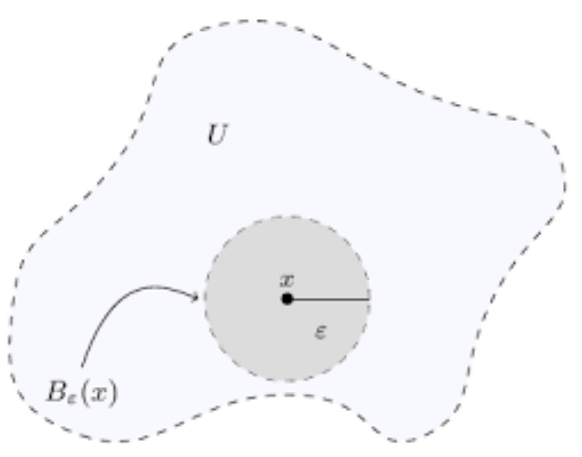
\includegraphics[width=8cm]{images/open_set.png}
    \caption{Open set}
\end{figure}

\section{Compactness}
\begin{defn}{Open cover}{}
By an \textbf{open cover} of a set $A$ in a metric space $X$ we mean a collection $\{G_\alpha\}$ of open subsets of $X$ such that $A \subset \bigcup_\alpha G_\alpha$.
\end{defn}

\begin{defn}{Compact set}{}
A subset $K$ of a topological (or metric) space is compact if every open cover of $K$ has a \emph{finite} subcover.
\end{defn}

An open cover of $A$ is a collection of open sets that collectively cover $A$.

A subcover is a subcollection of these open sets that still collectively cover $A$.

This means that any infinite collection of open sets that together cover a compact set always ``overcovers" it.

The simplest kind of compact set is just a finite set: a collection of finitely many points.


\section{Structures on Euclidean Space}\todo{to remove}
\begin{defn}{Limit and isolated point}{}
A point $p$ is a limit point of $E$ if every neighborhood of $p$ contains a point $q \neq p \in E$. 

If $p$ is not a limit point but is in $E$, then $p$ is an isolated point.
\end{defn}

\begin{defn}{Closed set}{}
$E$ is closed if every limit point of $E$ is in $E$. Intuitively, this means $E$ ``contains all its edges".

The closure $\bar{E}$ of $E$ is the union of E and the set of its limit points.
\end{defn}

\begin{defn}{Interior point}{}
A point $p$ is an interior point of $E$ if there is a neighborhood $N$ of $p$ such that $N \subset E$. Note that interior points must be in $E$ itself, while limit points need not be.
\end{defn}

\begin{defn}{Open set}{}
E is open if every point of E is an interior point of E. Intuitively, E “doesn’t have edges”.
\end{defn}

\begin{defn}{Dense set}{}
E is dense in X if every point of X is a limit point of E or a point of E, or both.
\end{defn}

\begin{defn}{Interior}{}
The interior $E^0$ of $E$ is the set of all interior points of $E$, or equivalently the union of all open sets contained in $E$.
\end{defn}

% https://www.dpmms.cam.ac.uk/~twk/Top.pdf

\chapter{Knot Theory}
\textbf{Readings:}
\begin{itemize}
\item \href{https://stanford.edu/~sfh/knot.pdf}{Knot Theory by Stanford University}
\item \href{https://www.math.cuhk.edu.hk/course_builder/1920/math4900e/Adams--The%20Knot%20Book.pdf}{The Knot Book by Colin C. Adams}
\end{itemize}

\section{Knot and Knot Types}
